\textbf{MIMO} (or \textbf{m}ultiple-\textbf{i}nput and \textbf{m}ultiple-\textbf{o}utput) is a technology that uses multiple antennas to increase the capacity of a wireless link. 
It is a key technology in modern wireless communication systems, including 4G networks and Wi-Fi. 
MIMO technology takes advantage of \textbf{multi-path propagation}, which means that signals can take multiple paths between the transmitter and receiver caused by reflections, diffractions, and scattering. 
By using multiple antennas at both the transmitter and receiver, MIMO technology can exploit these multiple paths to increase the data rate and reliability of the wireless link.

\begin{figure}[H]
	\centering
	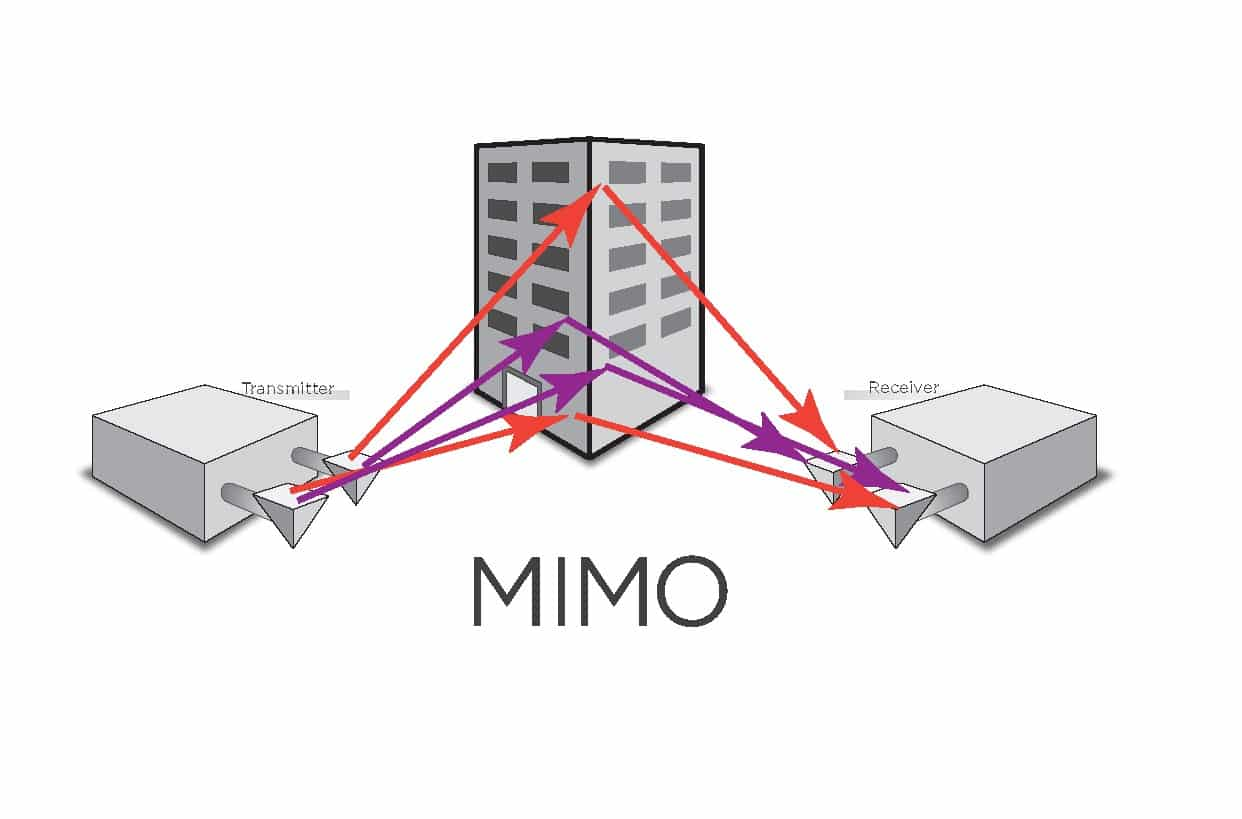
\includegraphics[width=0.4\textwidth]{Figures/mimo.png}
	\caption{Multiple-Input Multiple-Output (MIMO) system} 
\end{figure}

A early predecessor of MIMO technology is \textbf{Space-division multiple access} (SDMA), which used directional antennas to reach multiple users in different directions on the same frequency-band. MIMO technology, on the other hand, uses multiple antennas to transmit multiple data streams on the same frequency-band to the same user.


\subsection{Functions of MIMO}

\paragraph{Channel State Information (CSI)}
Channel State Information (CSI) refers to the knowledge of the communication channel’s characteristics, including attenuation, delay, and fading. 
It helps optimize transmission by adjusting power, phase, and modulation. 
CSI is estimated at the receiver and sent back to the transmitter. 
Accurate CSI is essential for techniques like beamforming and precoding to enhance signal strength and reduce interference.


\paragraph{Precoding and Beamforming}
Precoding is multi-stream beamforming that occurs at the transmitter. 
Beamforming adjusts phase and gain to maximize signal power at the receiver. 
It increases signal strength and reduces multipath fading. 
Precoding with multiple streams is useful when the receiver has multiple antennas and requires CSI.

\paragraph{Spatial Multiplexing}
Spatial multiplexing splits a high-rate signal into lower-rate streams, each transmitted from a different antenna. 
The receiver can separate the streams if it has accurate CSI. 
This technique increases capacity, especially at high SNR. 
The number of streams is limited by the smaller antenna count. 
It can work without CSI at the transmitter and can also support multi-user MIMO with CSI.

\paragraph{Diversity Coding}
Diversity coding transmits a single stream with space-time coding for reliability. 
It exploits independent fading across antennas but does not provide beamforming gains. 
When some CSI is available, diversity coding can combine with spatial multiplexing to improve performance.


\subsection{Variations of MIMO}

Different variations of MIMO systems include:

\begin{itemize}
    \item \textbf{Single-User MIMO (SU-MIMO):} 
    A MIMO system where multiple antennas are used at both the transmitter and receiver to improve data rates and reliability for a single user, using spatial multiplexing to transmit multiple data streams simultaneously.
    
    \item \textbf{Multi-User MIMO (MU-MIMO):} 
    Allows a base station to communicate with multiple users simultaneously, each with multiple antennas. This technique increases system capacity by enabling space-division multiple access (SDMA) based on spatial signatures of the users.
    
    \item \textbf{Massive MIMO:} 
    Involves a large number of antennas at the base station to serve many users simultaneously, greatly enhancing spectral and energy efficiency by exploiting spatial diversity.
    
    \item \textbf{Distributed MIMO:} 
    Utilizes multiple geographically separated antennas connected by a backhaul network, improving coverage and reliability over large areas by exploiting spatial diversity.
    
    \item \textbf{Cooperative MIMO:} 
    Involves collaboration between multiple devices (such as users or base stations) to transmit and receive signals, forming a virtual antenna array. This improves system performance through coordinated resource sharing.
\end{itemize}

\subsection{Antenna Configurations}

The amount of antennas used in a MIMO system on transmitter and receiver is referred to as the antenna configuration. 
Common configurations include 2x2, 4x4, 8x8, etc., where the first number represents the number of antennas on the transmitter and the second number represents the number of antennas on the receiver.
\begin{figure}[H]
	\centering
	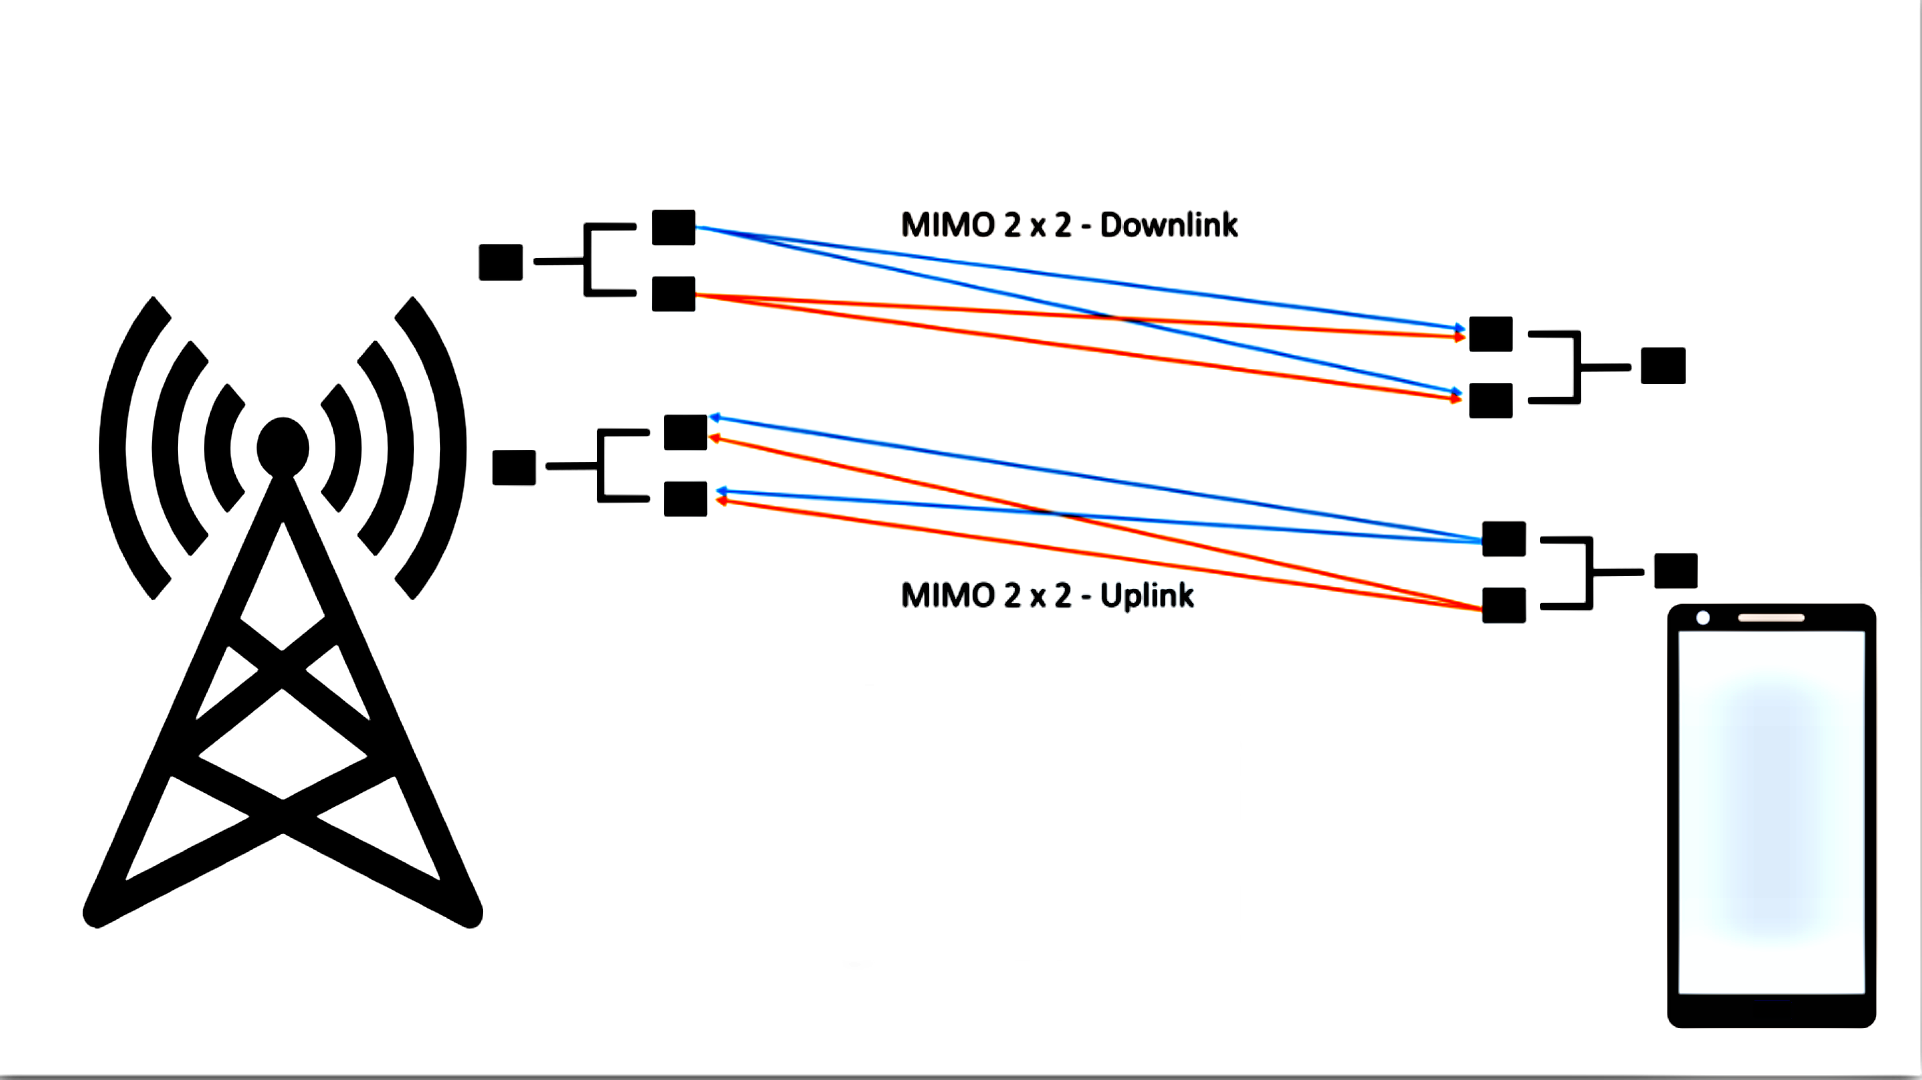
\includegraphics[width=0.6\textwidth]{Figures/mimo2x2.png}
	\caption{MIMO 2x2 Uplink and Downlink} 
\end{figure}

\subsubsection{MIMO in 4G Networks}

The 3rd Generation Partnership Project (3GPP) has defined different MIMO configurations for LTE, LTE Advanced, and LTE Advanced Pro networks.

\begin{table}[H]
    \centering
    \begin{tabular}{|l|l|l|}
    \hline
    \textbf{LTE Technology}      & \textbf{3GPP Release} & \textbf{Antenna Configuration (MIMO)} \\ \hline
    LTE                          & Release 8             & 4 x 4 Downlink \newline 2 x 2 Uplink  \\ \hline
    LTE Advanced                 & Release 10            & 8 x 8 Downlink \newline 4 x 4 Uplink  \\ \hline
    LTE Advanced Pro             & Release 13            & 8 x 8 Downlink \newline 4 x 4 Uplink  \\ \hline
    \end{tabular}
    \caption{MIMO configurations in LTE networks}
\end{table}
    